%=============================================================================
% Chapter 6: Structures
%=============================================================================
\chapter{Structures}
\label{ch:structures}

%-----------------------------------------------------------------------------
\section{Introduction to Structures}
\label{sec:struct-intro}
%-----------------------------------------------------------------------------

\begin{definitionbox}{Structure}
A \textbf{structure} groups several data items together to form a
single entity using the \texttt{struct} keyword.  Unlike arrays, the
members of a structure can be of \emph{different} data types.
\end{definitionbox}

\noindent
The general form for defining a structure is:

\begin{cppcode}
struct struct_name {
    data_type member1;
    data_type member2;
    // ...
    data_type memberN;
};
\end{cppcode}

\begin{importantbox}{Semicolon After the Closing Brace}
The closing brace of a \texttt{struct} definition \emph{must} be
followed by a semicolon.  Omitting it is one of the most common
syntax errors when working with structures.
\end{importantbox}

%-----------------------------------------------------------------------------
\section{Declaring Structures}
\label{sec:struct-declaring}
%-----------------------------------------------------------------------------

There are three common methods for declaring structure variables in C++.

\subsection{Method A --- Define First, Declare Later}

Define the structure type and then declare variables of that type
inside a function:

\begin{cppcode}
struct data {
    char *name;
    int age;
};

int main() {
    struct data student;      // declare variable of type 'data'
    student.name = "Ahmed";
    student.age  = 20;
    return 0;
}
\end{cppcode}

\subsection{Method B --- Define and Declare Together}

Declare one or more variables at the same time as the structure
definition:

\begin{cppcode}
struct data {
    char *name;
    int age;
} student;                   // 'student' is declared immediately

int main() {
    student.name = "Ahmed";
    student.age  = 20;
    return 0;
}
\end{cppcode}

\subsection{Method C --- Using \texttt{typedef}}

The \texttt{typedef} keyword creates an alias for the structure type,
allowing variables to be declared without the \texttt{struct} keyword:

\begin{cppcode}
typedef struct {
    char *name;
    int age;
} Student;                   // 'Student' is now a type alias

int main() {
    Student s1, s2;          // no 'struct' keyword needed
    s1.name = "Ahmed";
    s1.age  = 20;
    return 0;
}
\end{cppcode}

\begin{infobox}{The Dot Operator}
Structure members are accessed using the \textbf{dot operator}
(\texttt{.}).  The syntax is:

\medskip
\texttt{variable\_name.member\_name}
\medskip

For example: \texttt{student.name = "Ahmed";} and
\texttt{student.age = 20;}
\end{infobox}

\begin{conceptbox}{\texttt{typedef} and Multiple Names}
With \texttt{typedef} you can create multiple convenient aliases for
the same structure.  This is especially useful when porting code
across different projects or when you want shorter type names.
\end{conceptbox}

%-----------------------------------------------------------------------------
\section{Practical Examples}
\label{sec:struct-examples}
%-----------------------------------------------------------------------------

\subsection{Example 1 --- Parts Inventory}

A structure to represent a single part in an inventory system:

\begin{cppcode}
#include <iostream>
using namespace std;

struct part {
    int   model_no;
    int   part_no;
    float cost;
};

int main() {
    struct part p1;

    cout << "Enter model number: ";
    cin  >> p1.model_no;
    cout << "Enter part number:  ";
    cin  >> p1.part_no;
    cout << "Enter cost:         ";
    cin  >> p1.cost;

    cout << "\n--- Part Details ---" << endl;
    cout << "Model No : " << p1.model_no << endl;
    cout << "Part No  : " << p1.part_no  << endl;
    cout << "Cost     : " << p1.cost     << endl;

    return 0;
}
\end{cppcode}

\noindent
\textbf{Sample run:}
\begin{verbatim}
Enter model number: 101
Enter part number:  5042
Enter cost:         29.95

--- Part Details ---
Model No : 101
Part No  : 5042
Cost     : 29.95
\end{verbatim}

\subsection{Example 2 --- Adding Distances (English System)}

In the English measurement system, distances are expressed in feet and
inches.  The following program adds two distances:

\begin{cppcode}
#include <iostream>
using namespace std;

struct distance {
    int   feet;
    float inches;
};

int main() {
    distance d1, d2, d3;

    // Input first distance
    cout << "Enter feet for d1: ";   cin >> d1.feet;
    cout << "Enter inches for d1: "; cin >> d1.inches;

    // Input second distance
    cout << "Enter feet for d2: ";   cin >> d2.feet;
    cout << "Enter inches for d2: "; cin >> d2.inches;

    // Add the two distances
    d3.inches = d1.inches + d2.inches;
    d3.feet   = d1.feet   + d2.feet;

    // Handle carry: 12 inches = 1 foot
    if (d3.inches >= 12.0) {
        d3.inches -= 12.0;
        d3.feet   += 1;
    }

    cout << "\nSum = " << d3.feet << " feet, "
         << d3.inches << " inches" << endl;

    return 0;
}
\end{cppcode}

\noindent
\textbf{Sample run:}
\begin{verbatim}
Enter feet for d1: 5
Enter inches for d1: 8.5
Enter feet for d2: 3
Enter inches for d2: 7.2

Sum = 9 feet, 3.7 inches
\end{verbatim}

%-----------------------------------------------------------------------------
\section{Structures within Structures}
\label{sec:struct-nested}
%-----------------------------------------------------------------------------

Structures can be \emph{nested}: a member of one structure can itself
be another structure.  This is useful for modelling real-world entities
that are composed of sub-entities.

\subsection{Example 3 --- Room Area with Nested Distances}

\begin{cppcode}
#include <iostream>
using namespace std;

struct distance {
    int   feet;
    float inches;
};

struct room {
    distance length;
    distance width;
};

int main() {
    room dining;

    // Input length
    cout << "Enter length (feet): ";
    cin  >> dining.length.feet;
    cout << "Enter length (inches): ";
    cin  >> dining.length.inches;

    // Input width
    cout << "Enter width (feet): ";
    cin  >> dining.width.feet;
    cout << "Enter width (inches): ";
    cin  >> dining.width.inches;

    // Convert to total inches for area calculation
    float len = dining.length.feet * 12 + dining.length.inches;
    float wid = dining.width.feet  * 12 + dining.width.inches;

    float area_sqin = len * wid;
    float area_sqft = area_sqin / 144.0;  // 144 sq inches = 1 sq foot

    cout << "\nRoom area = " << area_sqft
         << " square feet" << endl;

    return 0;
}
\end{cppcode}

\noindent
\textbf{Sample run:}
\begin{verbatim}
Enter length (feet): 12
Enter length (inches): 6.5
Enter width (feet): 10
Enter width (inches): 3.0

Room area = 128.854 square feet
\end{verbatim}

\begin{conceptbox}{Accessing Nested Members}
When structures are nested, you chain the dot operator to reach inner
members:

\medskip
\texttt{dining.length.feet} \quad
\texttt{dining.length.inches} \quad
\texttt{dining.width.feet} \quad
\texttt{dining.width.inches}
\medskip

Each dot moves one level deeper into the structure hierarchy.
\end{conceptbox}

\noindent
The nesting relationship can be visualised as follows:

\begin{center}
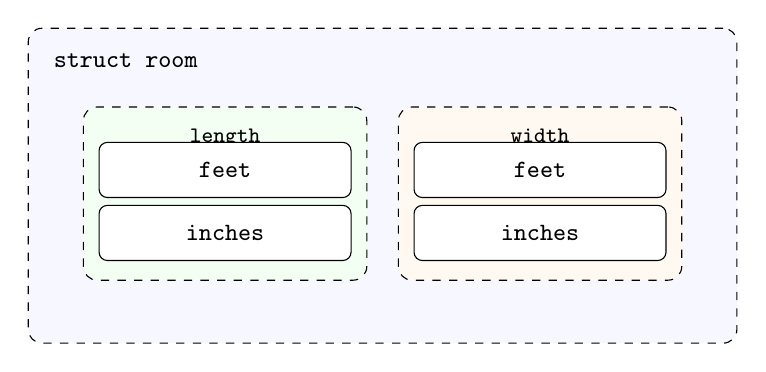
\begin{tikzpicture}[
    box/.style={draw, rounded corners=3pt, minimum width=3.2cm,
                minimum height=0.7cm, font=\small\ttfamily},
    outer/.style={draw, rounded corners=5pt, dashed, inner sep=10pt,
                  fill=blue!3},
    arr/.style={->, >=stealth, thick}
]
  % Room box
  \node[outer, minimum width=9cm, minimum height=4cm] (roombox) at (0,0) {};
  \node[font=\bfseries\small, anchor=north west] at (-4.3,1.8)
       {\texttt{struct room}};

  % Length
  \node[outer, minimum width=3.6cm, minimum height=2.2cm, fill=green!5]
       (lenbox) at (-2, -0.1) {};
  \node[font=\footnotesize\bfseries, anchor=north] at (-2, 0.85)
       {\texttt{length}};
  \node[box, fill=white] at (-2, 0.2) {feet};
  \node[box, fill=white] at (-2,-0.6) {inches};

  % Width
  \node[outer, minimum width=3.6cm, minimum height=2.2cm, fill=orange!5]
       (widbox) at (2, -0.1) {};
  \node[font=\footnotesize\bfseries, anchor=north] at (2, 0.85)
       {\texttt{width}};
  \node[box, fill=white] at (2, 0.2) {feet};
  \node[box, fill=white] at (2,-0.6) {inches};
\end{tikzpicture}
\end{center}

%-----------------------------------------------------------------------------
\section{Array of Structures}
\label{sec:struct-array}
%-----------------------------------------------------------------------------

\begin{definitionbox}{Array of Structures}
Since a \texttt{struct} defines a new data type, you can create an
\textbf{array of structures} just as you would create an array of
\texttt{int} or \texttt{float}.  Each element of the array is a
complete structure with all its members.
\end{definitionbox}

\noindent
The conceptual layout of an array of structures is shown below:

\begin{center}
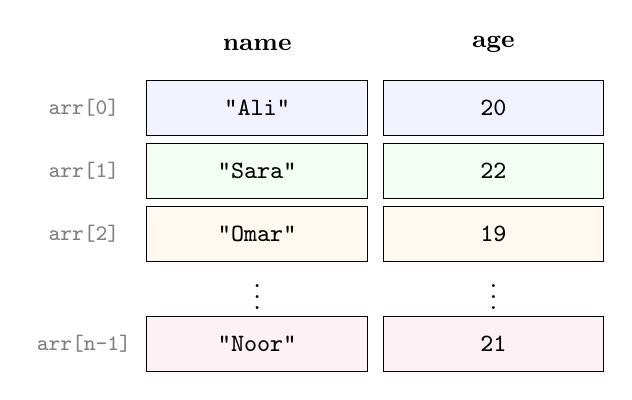
\begin{tikzpicture}[
    cell/.style={draw, minimum width=2.8cm, minimum height=0.7cm,
                 font=\small\ttfamily},
    idx/.style={font=\footnotesize\ttfamily, text=gray}
]
  % Column headers
  \node[font=\small\bfseries] at (0, 1.2)  {name};
  \node[font=\small\bfseries] at (3, 1.2)  {age};

  % Row 0
  \node[cell, fill=blue!5]   at (0, 0.4) {"Ali"};
  \node[cell, fill=blue!5]   at (3, 0.4) {20};
  \node[idx] at (-2.2, 0.4)  {arr[0]};

  % Row 1
  \node[cell, fill=green!5]  at (0, -0.4) {"Sara"};
  \node[cell, fill=green!5]  at (3, -0.4) {22};
  \node[idx] at (-2.2,-0.4)  {arr[1]};

  % Row 2
  \node[cell, fill=orange!5] at (0, -1.2) {"Omar"};
  \node[cell, fill=orange!5] at (3, -1.2) {19};
  \node[idx] at (-2.2,-1.2)  {arr[2]};

  % dots
  \node at (0, -1.9) {$\vdots$};
  \node at (3, -1.9) {$\vdots$};

  % Row n-1
  \node[cell, fill=purple!5] at (0, -2.6) {"Noor"};
  \node[cell, fill=purple!5] at (3, -2.6) {21};
  \node[idx] at (-2.2,-2.6)  {arr[n-1]};
\end{tikzpicture}
\end{center}

\subsection{Example 4 --- Array of Student Structures}

\begin{cppcode}
#include <iostream>
#include <cstring>
using namespace std;

struct student {
    char name[30];
    int  age;
};

int main() {
    const int SIZE = 3;
    student arr[SIZE];

    // Input
    for (int i = 0; i < SIZE; i++) {
        cout << "Enter name of student " << i + 1 << ": ";
        cin.getline(arr[i].name, 30);
        cout << "Enter age of student " << i + 1 << ":  ";
        cin  >> arr[i].age;
        cin.ignore(80, '\n');   // flush newline
    }

    // Output
    cout << "\n--- Student List ---" << endl;
    for (int i = 0; i < SIZE; i++) {
        cout << "Student " << i + 1 << ": "
             << arr[i].name << ", Age: "
             << arr[i].age  << endl;
    }

    return 0;
}
\end{cppcode}

\noindent
\textbf{Sample run:}
\begin{verbatim}
Enter name of student 1: Ali Hassan
Enter age of student 1:  20
Enter name of student 2: Sara Karim
Enter age of student 2:  22
Enter name of student 3: Omar Faris
Enter age of student 3:  19

--- Student List ---
Student 1: Ali Hassan, Age: 20
Student 2: Sara Karim, Age: 22
Student 3: Omar Faris, Age: 19
\end{verbatim}

\begin{infobox}{Accessing Members of Array Elements}
Use the array subscript followed by the dot operator:

\medskip
\texttt{arr[i].name} \qquad \texttt{arr[i].age}
\medskip

This first selects element \texttt{i} from the array and then
accesses the desired member of that element's structure.
\end{infobox}

\begin{conceptbox}{Structures vs.\ Arrays}
\renewcommand{\arraystretch}{1.3}
\begin{tabular}{@{} p{6.5cm} p{6.5cm} @{}}
\toprule
\textbf{Array} & \textbf{Structure} \\
\midrule
All elements must be of the \emph{same} data type.
    & Members can be of \emph{different} data types. \\
Elements are accessed by \textbf{index} (e.g.\ \texttt{a[0]}).
    & Members are accessed by \textbf{name} (e.g.\ \texttt{s.age}). \\
Useful for storing a collection of \emph{similar} items (e.g.\ 100
    marks). & Useful for grouping \emph{related but different}
    attributes (e.g.\ name, age, GPA). \\
Cannot be assigned directly with \texttt{=} in C-style arrays.
    & Can be assigned directly: \texttt{s2 = s1;} copies all members. \\
Fixed-size, determined at compile time.
    & Each variable holds one complete set of members. \\
\bottomrule
\end{tabular}
\end{conceptbox}
